% -*- mode: latex-mode; TeX-engine: xetex; LaTeX-command-style: (("" "SOURCE_DATE_EPOCH=0 %(PDF)%(latex) --shell-escape %S%(PDFout)")); TeX-master: "../dissertation.tex"; -*-

\chapter{Loading of Single Atoms in Optical Tweezer}
\label{ch:loading}

\section{Introduction}
\label{ch:loading:introduction}

The atoms we use in the experiment comes from alkali metal dispensers
heated using an electric current which have a starting temperature of
$\approx400\sim800~\mathrm{K}$ and must be cooled to $<0.1~\mathrm{K}$
before they can be captured by the optical tweezer.
In this chapter, we will breifly discuss the cooling steps that bridge this temperature gap.
In section \ref{ch:loading:free-space}, we will focus on the free space cooling
on the atoms without involving the optical tweezer.
Since most of the cooling techniques used in our experiment are quite standard,
they will not be reviewed in detail here.
Instead, we will mainly highlight the important specific design choices
and their performance in our experiment as reference.
Section \ref{ch:loading:loading} will discuss the loading and detection
of the atom in the tweezer including a short summary of the unique challenge
we face with Na atoms.

\section{Free Spacing Cooling of Atoms}
\label{ch:loading:free-space}

\begin{figure}
  \centering
  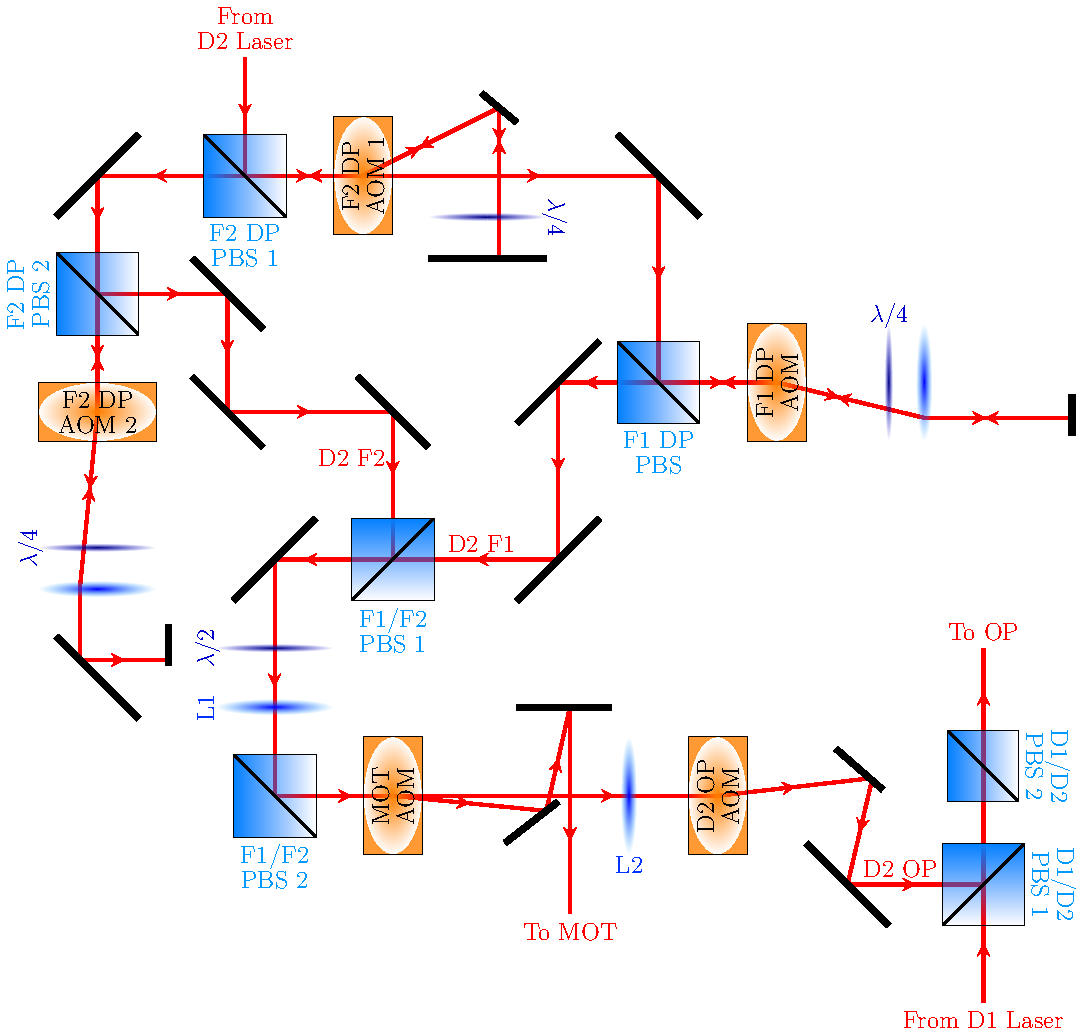
\includegraphics[width=\textwidth]{figures/loading_na_res_beampath.pdf}
  \caption[Beampath for Na D1 and D2 light.]{
    Beampath for generating the frequencies for Na MOT and optical pumping~(OP).
    (Beampath for fiber coupling and frequency locking is not shown.
    The power control for the D1 laser is also omitted.)
    The D2 laser is locked on the F1/F2 crossover line using
    saturated absorption locking\todo{ref}.
    It is shifted down by the two F2 double-pass~(DP) AOMs to generate the frequency
    for the Na $F=2$ state and shifted up by the F1 DP AOM to address the Na $F=1$ state.
    The frequencies of the F1/F2 light are controlled by the F1 DP AOM
    and F2 DP AOM 2 respectively.
    This set up makes sure that when the F1/F2 DP AOMs are off,
    the closest frequency in the leaked light is at least detuned
    by half the F1/F2 separation~($\approx880~\mathrm{MHz}$)~\cite{steck_sodium_2019}
    and will have minimum effect on the atom.
    The F1 and F2 light are combined on F1/F2 PBS 1 and their power ratio after the
    F1/F2 PBS 2 is controlled by the half waveplate between the two PBSs.
    A similar setup is used to combine the D1 and D2 light in the OP output using
    D1/D2 PBS 1 and the rotating D1/D2 PBS 2.
    Since we need to switch the Na MOT light on and off out-of-phase
    with the Na tweezer~\cite{hutzler_eliminating_2017} at a high frequency,
    the sharpness of the turn on/off edge in the MOT AOM is important.
    We focus the beam through the AOM using lens L1 to optimize the switching time.
    This is then collimated by lens L2 for the downstream beampath.
    \label{fig:loading:free-space:na-res-beampath}}
\end{figure}

\begin{figure}
  \centering
  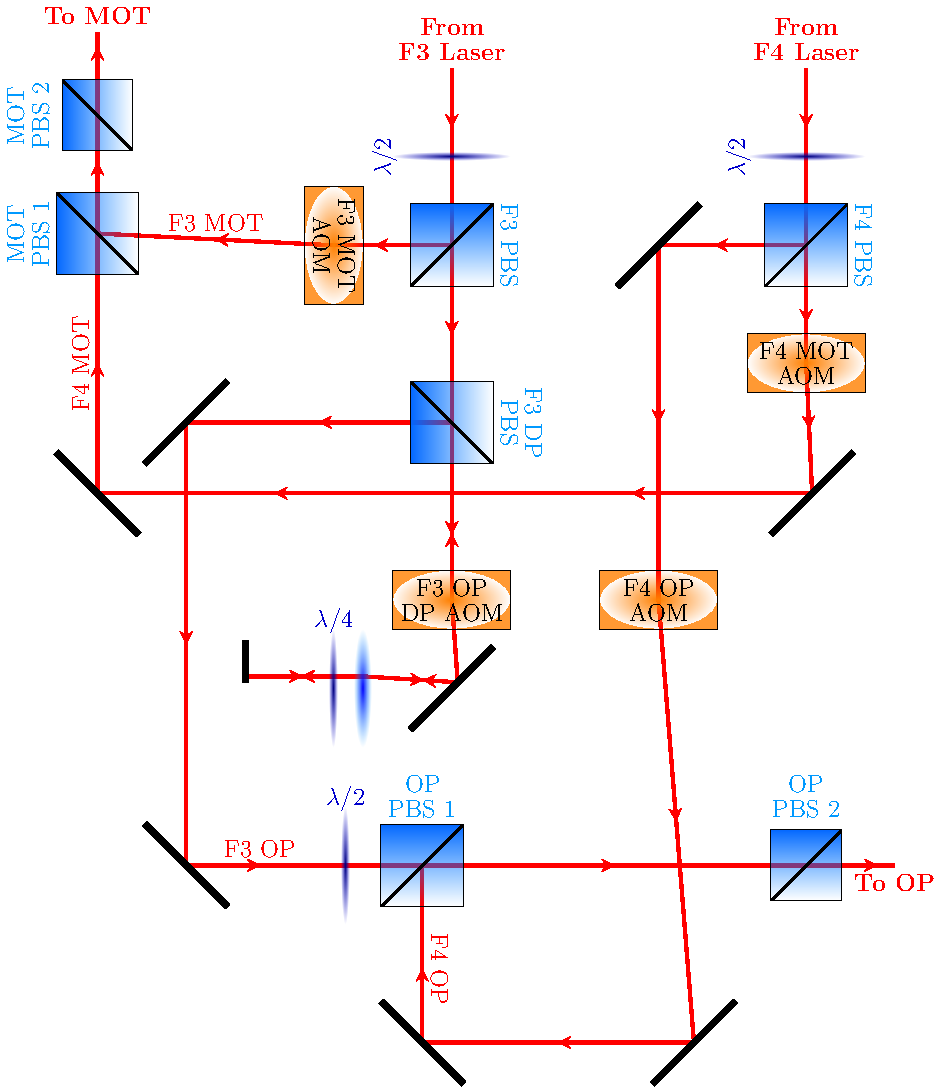
\includegraphics[width=0.866\textwidth]{figures/loading_cs_res_beampath.pdf}
  \caption[Beampath for Cs D2 light.]{
    Beampath for generating the frequencies for Cs MOT and optical pumping~(OP).
    (Beampath for fiber coupling and frequency locking is not shown.)
    The F3 laser is locked using saturated absorption locking
    to the F3 atomic transition.
    The F4 laser is beat-locked to the F3 laser, which also controls its frequency.
    The F3 and F4 light are combined on MOT PBS 1 and OP PBS 1
    and their power ratio in the MOT and OP output are controlled by the
    rotating MOT PBS 2 and OP PBS 2 respectively.
    The frequency of the F3 light in the MOT is fixed whereas
    the frequency of the F3 light in the OP is can be changed by the F3 OP DP AOM.
    \label{fig:loading:free-space:cs-res-beampath}}
\end{figure}

Our experiment begins with the loading of a Na Cs dual species magneto-optical trap~(MOT)
from the background pressure created by the dispensers.
It is created using six cooling beams of $\approx\todo{number}~\mathrm{mm}$ diameter
with $\approx\todo{number}~\mathrm{mW}$~(Na) and $\approx\todo{number}~\mathrm{mW}$~(Cs)
power in each beams.
The resulting MOT has a diameter of $\approx\todo{number}~\mathrm{mm}$
with $\approx\todo{number}$~(Na) and $\approx\todo{number}$~(Cs) atoms being trapped
and cooled to to a temperature of $\approx\todo{number}~\mathrm{mK}$~(Na)
and $\approx\todo{number}~\mathrm{mK}$~(Cs).
The atom numbers are significantly smaller than the ones typically seen in a bulk gas experiment
since the goal of the free-space laser cooling is to load atoms into the tweezers
which does not require large atom numbers.
The small size of the MOT requires a tigher tolerance on the MOT position
in order to overlap with the optical tweezer for the loading of single atoms,
which in turns increased the sensitivity to to the alignment
and power balance of the cooling beams that determines the MOT position.
Because of this, we use four independent fibers to deliver the power
for the four horizontal cooling beams which allows independent control
of the power and alignment.
We observed a more robust MOT and, as a result, single atom loading
compared to using retro-reflectors to create conterpropagating horizontal cooling beams.
Due to the geometric constraints in the experiment,
retro-reflector is used for verticle cooling beams.

The MOT is followed by a compressed-MOT~(CMOT) stage for Na
which uses light closer to resonant to push the Na atoms closer to the center
as well as reducing their temperature to $\approx\todo{number}~\mathrm{mK}$.
After this, the magnetic field is turned off and
a polarization gradient cooling step is applied on the atoms
which cools the atoms to $\approx\todo{number}~\mathrm{mK}$~(Na)
and $\approx\todo{number}~\mathrm{mK}$~(Cs).

The beampaths for generating all the necessary frequencies are shown in
Fig.~\ref{fig:loading:free-space:na-res-beampath}~(Na) and
Fig.~\ref{fig:loading:free-space:cs-res-beampath}~(Cs).
The same beampaths are also used for generating the light for cooling
and imaging of single atoms as well as optical pumping for state preparation
that will be discussed in later chapters.

\section{Loading and Imaging in the Tweezer}
\label{ch:loading:loading}

We load the tweezer from the laser cooled cloud of atoms.
Since the tweezer provides a conservative potential,
trapping of the atom requires its energies to be reduced.
This can be done either by changing the trap depth,
e.g. turning on the trap when an atom is at the focus to reduce its potential energy,
or by a dissipative cooling process.
Given the density of the MOT, there is less than $\todo{...}$ atom in the trap volume,
so the only method that works for loading tweezer in our experiment
is by cooling the atoms into the tweezer.
The cooling process also ensure that at most one atom can be loaded into the tweezer
due to pair-wise loss from light-assisted collision.\todo{cite}

Cooling in tweezer and loading using the free-space cooling beams works well for Cs.
However, the cooling of Na atoms in the tweezer is more challenging
due to the light shift from the tweezer.
The higher trap depth necessary to trap the hotter Na atom after freespace cooling
and the absense of an accessible magic wavelength causes a large (\todo{number?})
light shift on the cooling transition when the Na atom is in the tweezer.
This shift significantly changes the cooling detuning making it ineffective in the tweezer.
We fix this issue by alternating the cooling and the tweezer light at $2.5~\mathrm{MHz}$.
The frequency is low enough to allow a few photon to be scattered
when the cooling light is on to perform cooling on the atom,
yet high enough compared to the highest trapping frequency in the tweezer
to prevent parametric heating of the trapped atom.\todo{cite}

\todo{
\item Need cooling in tweezer
\item Need switching tweezer for Na
\item Additional trap depth constraint due to imaging
\item Tweezer parameter
  NA, waist, power calibration (for the rest of the thesis), uncertainty
  (guarantee loading of atoms in respective tweezer)
\item Can load atom and MOT-free atom image

  Moreover, we use florescence imaging to detect the atoms in the tweezer
  which also requires cooling to prevent the recoil from heating the atom out of the tweezer
  before enough photons can be collect.
  We can estimate the the requirement of the cooling as follows.
}
\todo{
  cite Lee's thesis
}

\section{Summary and Outlook}
\label{ch:loading:summary}

\todo{mention single photon imaging techniques?}

In this chapter we discussed the trapping and imaging of the single atoms in the optical
tweezers and the steps leading up to it.
We take advantage of many techniques developped and used in previous experiments
to boost our control on the atoms in preparation for the control on the molecules.

The atoms trapped in the tweezers and the high fidelity detection of them
form the fundation of our experiment.
The utility of such system and the possibility it opens up will be discussed
in more detail in the coming chapters.
